\chapter{Analýza požadavků}

Cílem nového skladového systému je nahradit a rozšířit funkce stávajícího skladového systému Sysel - proto jsme při analýze požadavků vycházeli\footnote{Já a kolega Pavel Kovář, který se zabývá backendem nového systému} jednak z tohoto řešení a dále z požadavků primárního potenciálního zákazníka - jednoho ze současných uživatelů tohoto systému.\\
Současná verze Sysla je již oproti svému původnímu návrhu velmi upravena, a to se podepisuje na snížené možnosti dalších úprav a celkové komplexnosti systému.\\
Pro nový systém je na jedné straně důležité, aby bylo stále možné provádět ty procesy, které jsou ideální již za současného stavu. Na straně druhé je pak důležité zohlednit nové požadavky a pokusit se umožnit i snadné reakce na budoucí požadavky.

\section{Analýza požadavků dle současného systému}

Jádrem současného skladového systému je rozdělení na dvě role: skladník a vedoucí. Aplikace podporuje práci ve středně velkém skladu, který používá čárové kódy na zboží a umístěních, ale nemá další pokročilé automatizace jako například pohyb objednávkových bedýnek po páse, roboty, kteří autonomně vyzvedávají zboží atp. Veškeré pohyby jsou realizovány lidskými zdroji a tomu odpovídá i realizace podpůrného systému. Výhodou tohoto řešení je možnost použití systému i v menších skladech a to případně i o velikostí pouze jednoho správce.\\
\\
\subsection{Funkční požadavky}

Role skladníka:
\begin{itemize}
	\item přijímat nové dodávky zboží,
	\item naskladňovat zboží,
	\item přesouvat zboží v rámci skladu,
	\item přesouvat celá umístění,
	\item vyskladňovat zboží,
	\item provést inventuru,
	\item zobrazovat úlohy.
\end{itemize}

Role vedoucího:
\begin{itemize}
	\item spravovat sklady,
	\item spravovat umístění ve skladech,
	\item spravovat výrobce,
	\item spravovat zboží,
	\item zadávat úlohy skladníkům,
	\item sledovat stav probíhajících a uzavřených úloh.
\end{itemize}

Tyto požadavky vychází ze stávající aplikace Sysel a jejich procesy měly zůstat zachovány, proto jsme konkrétní use-case a detailní procesy navrhli na základě průchodů současného systému. Diagramy, které jsou výstupem této části analýzy jsou součástí přílohy \ref{ap:diagram:storekeeper}.

\section{Analýza nových požadavků}

\subsection{Logistika}

Hlavním novým požadavkem, který současný Sysel nepodporuje, je správa \emph{Logistiky} - tedy místa ve skladu, kde dochází ke kompletaci odchozího zboží, jeho balení atp.\\
Toto místo se od běžného skladového umístění odlišuje v tom, co se zde navíc eviduje:
\begin{itemize}
	\item \emph{Použitý spotřební materiál} Zaznamenávají se spotřebované balíky či fólie, ale například i palety.
	\item \emph{Doba uložení} Ukládá se, jak dlouho zde dané zboží \uv{zabíralo} místo.
	\item \emph{Činnosti skladníka} Zde se eviduje, kolik a jaké úkony musel skladník se zbožím provést - jako například \emph{balení do folie}, \emph{přeskládání} atp.
\end{itemize}

\subsection{Evidence stráveného času}

Podobně jako se u Logistiky má ukládat čas, po který zboží leželo v Logistice, mělo by být možné v aplikaci celkově evidovat, kolik času strávil skladník jakým úkolem. Při přijetí úkolu se automaticky spustí stopky měřící strávený čas daným úkolem, také je ale nutné mít možnost stopky pozastavit - například během pauzy na oběd apod.\\
Časové přehledy skladníků by měly být použitelné jednak pro kontrolu výkonu skladníků, ale také pro potenciální fakturaci nákladů třetím stranám - pro případ, že by sklad provozoval jiný subjekt, než je reálný majitel zboží, který platí za uskladnění.

\subsection{Rozhraní pro nemobilní zařízení}

Současný systém je navržen mobile-first, což by mělo být zachováno - skladníci používají mobilní zařízení se zabudovanou čtečkou. Toto rozhraní se ale prakticky vůbec nezmění i při použití větší obrazovky - na tabletech je rozhraní ještě poměrně použitelné, ale na notebooku či stolním počítači je zobrazení přinejmenším \emph{neoptimalizované} - neexistuje zde žádná práce s horizontálním místem, vše je řazeno vertikálně. Jako ukázku přikládám screenshot úryvku domovské obrazovky vedoucího skladu (obrázek \ref{picture:sysel:vertical}), obsahující náhled na reálný stav používaného skladu, s anonymizovanými daty.\\
Požadavkem tedy je, aby rozhraní bylo plně responzivní - skladník sice typicky na počítači opravdu používán nebude, ale vedoucí skladu by měl mít možnost volně přecházet mezi různými zařízeními.

\begin{figure}[]
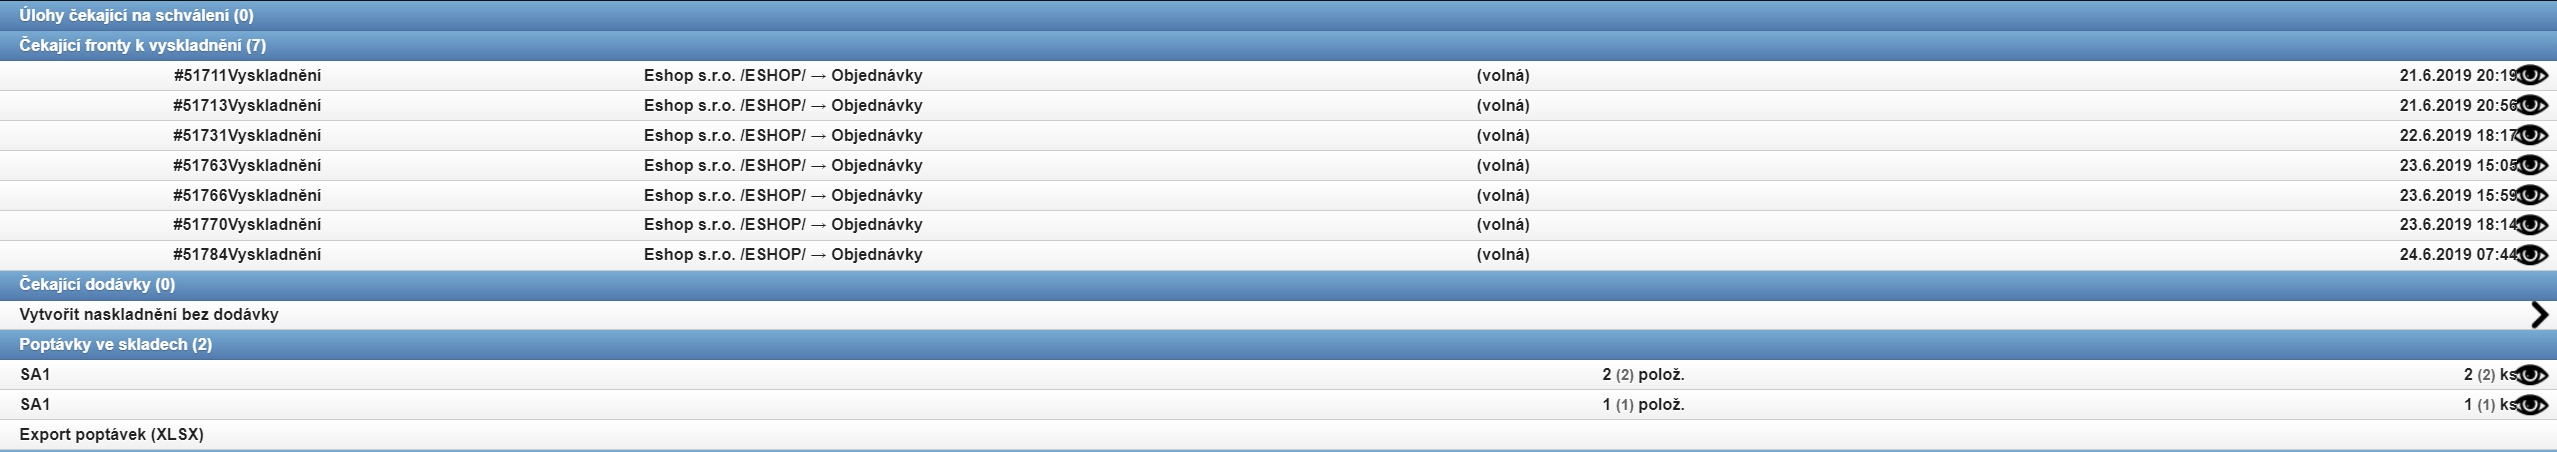
\includegraphics[width=\textwidth]{../png/sysel/vertical.png}
\caption{Ukázka špatné práce s horizontálním místem ve starém skladovém systému} \label{picture:sysel:vertical}
\end{figure}
